\frame{
	\frametitle{Workflow Overview}
	\only<1>{CAD design}
	\only<2>{STL Interface}
	\only<3>{Voxelization}
	\only<4>{TPD input file - Specification of loads and fixtures}
	\only<5>{Topology optimization}
	\only<6>{Voxelised geometry}
	\only<7>{Post-processing: Parametrization, Feature recognition}
	\begin{figure}
		\scalebox{0.14}{
\includegraphics{Pictures/1CAD.pdf}}
		\pause
		\scalebox{0.14}{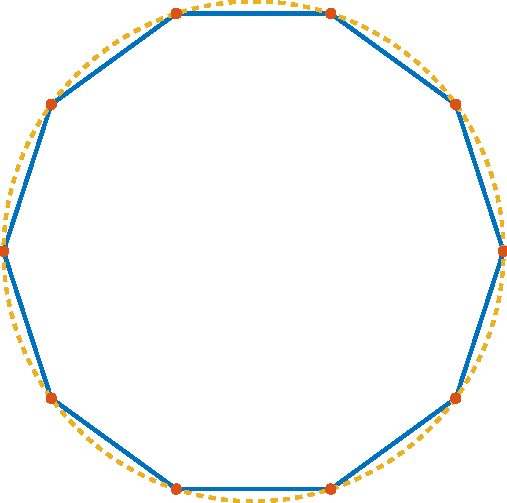
\includegraphics{Pictures/2STL.pdf}}
		\pause
		\scalebox{0.14}{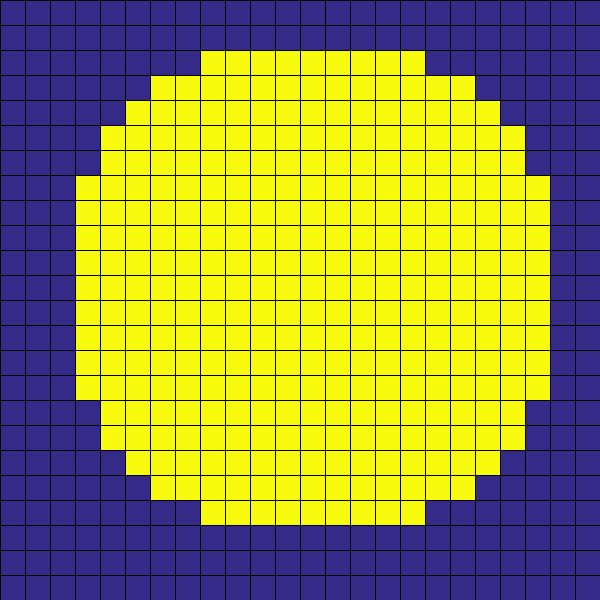
\includegraphics{Pictures/3VOX.pdf}}
		\pause
		\scalebox{0.14}{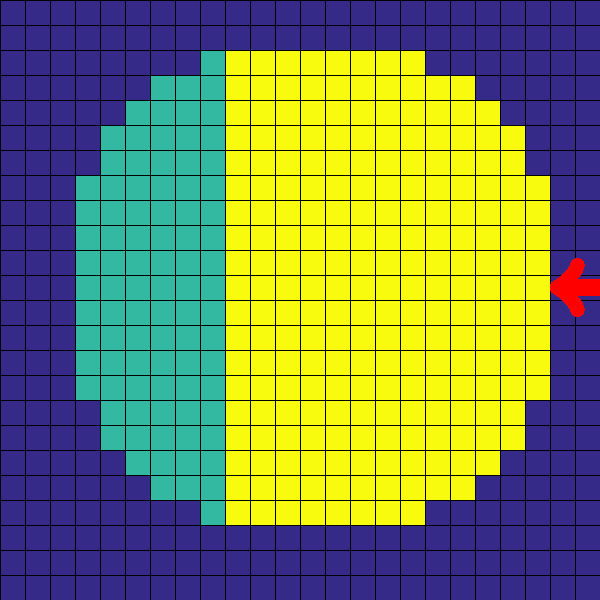
\includegraphics{Pictures/4TPD.pdf}}
		\pause
		\scalebox{0.14}{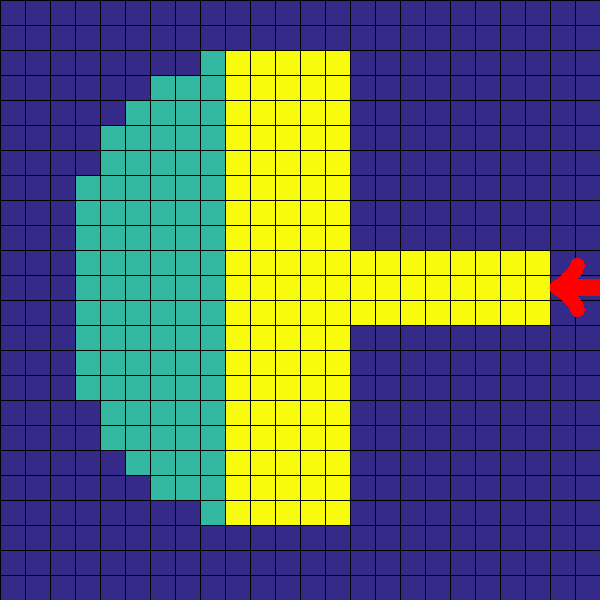
\includegraphics{Pictures/5TOPOPT.pdf}}
		\pause
		\scalebox{0.14}{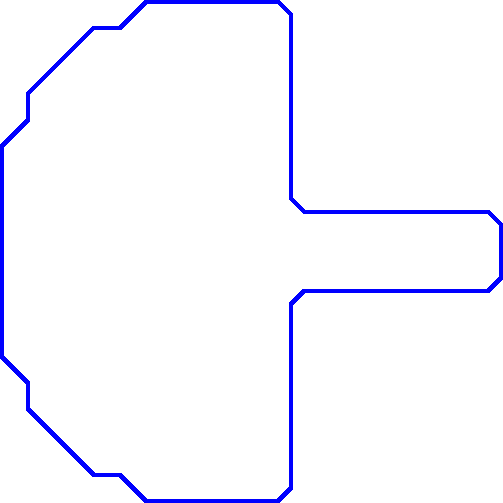
\includegraphics{Pictures/7MC.pdf}}
		\pause
		\scalebox{0.14}{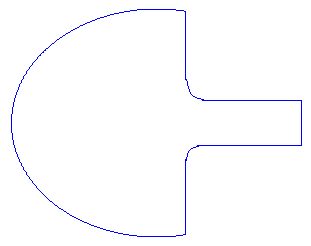
\includegraphics[scale=1.3]{Pictures/End.png}}
	\end{figure}
	\only<0>{CAD design}
	\only<2>{STL interface}
}
